\chapter{Evaluation}
This chapter shows the results of the experiment and how the gathered data can be interpreted. 

\subsection{output format}
Figure \ref{entries} shows the format of a single entry after the decryption. 

\begin{figure}[!htb]
\centering
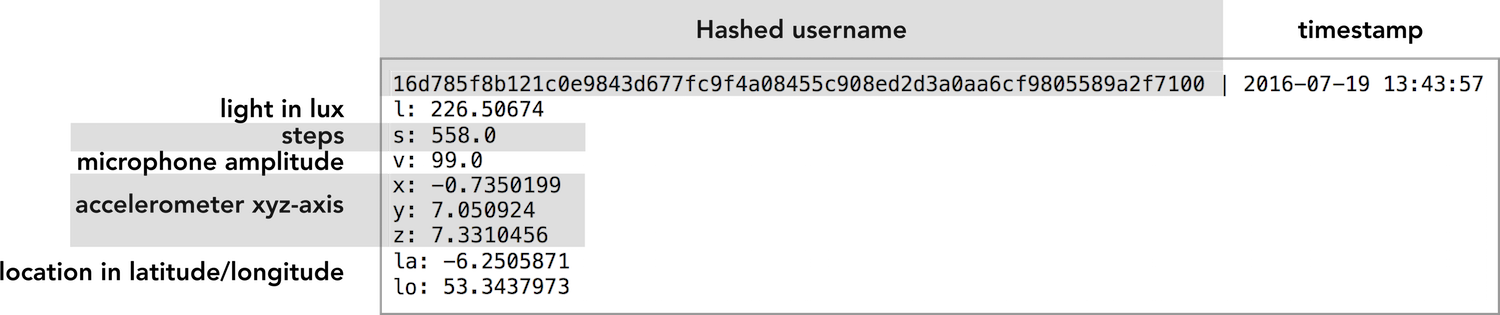
\includegraphics[width=\textwidth]{entries}
\caption{gathered data}\label{entries}
\vspace{10 mm}
\end{figure}

\FloatBarrier

\subsection{Results}
Participant number 2 was the only one who answered the question of being distracted during the experiment with 'yes'. Also the volume amplitude had some very high peeks that were not found in the measurements of other participants in that level \ref{volps}. 
\bigbreak
In the diagram \ref{ligps}, participant 1 is not mentioned. That is because the app wasn't able to access data from the light sensor. In the  measurements of the other participants it is again noticeable that Participant 2 shows different patterns than the others. The light value in lux differs from the others in it's dynamic. The value is much less constant and possibly an indicator, that it could influence the concentration in a negative way.\\
The detailed results are attached to this dissertation in Appendix 4.

%%%%%%% VOLUME
\begin{figure}[ht]
	\centering
	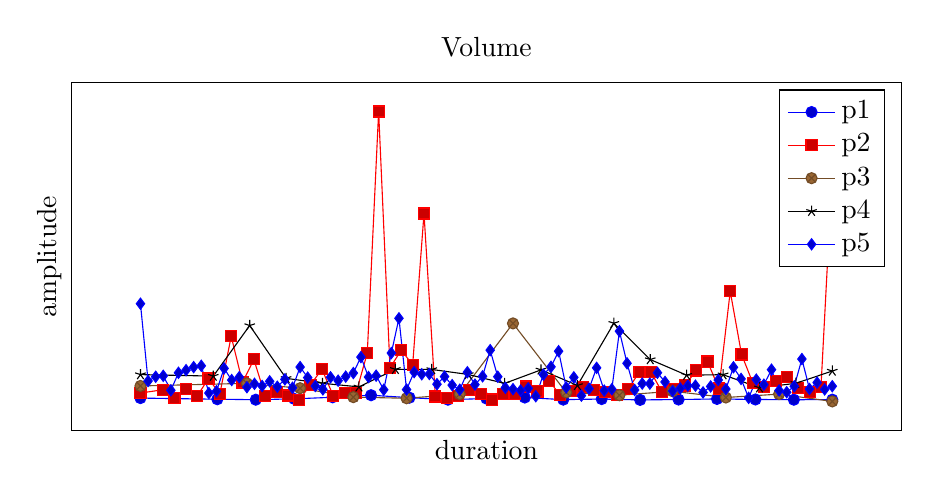
\begin{tikzpicture}
	\pgfplotsset{ticks=none}
\begin{axis}[
	height=6cm,
	width=\textwidth,
	ylabel=amplitude,
	xlabel=duration,
	title=Volume,
	unbounded coords=discard],
	
\addplot coordinates {
(0, 23.6857142857)
(10.1111111111, 15.5)
(15.1666666667, 12.1470588235)
(20.2222222222, 18.1212121212)
(25.2777777778, 29.3823529412)
(30.3333333333, 44.0294117647)
(35.3888888889, 26.5882352941)
(40.4444444444, 12.4411764706)
(45.5, 20.3636363636)
(50.5555555556, 27.7058823529)
(55.6111111111, 12.7058823529)
(60.6666666667, 16.7941176471)
(65.7222222222, 10.7352941176)
(70.7777777778, 13.2727272727)
(75.8333333333, 17.5882352941)
(80.8888888889, 13.7352941176)
(85.9444444444, 12.0882352941)
(91.0, 12.5)
};

\addplot coordinates {
(0, 59.5882352941)
(2.98360655738, 83.125)
(4.47540983607, 23.0)
(5.96721311475, 88.25)
(7.45901639344, 38.75)
(8.95081967213, 162.333333333)
(10.4426229508, 53.0)
(11.9344262295, 462.666666667)
(13.4262295082, 134.333333333)
(14.9180327869, 298.5)
(16.4098360656, 38.5)
(17.9016393443, 64.3333333333)
(19.393442623, 42.0)
(20.8852459016, 12.5)
(22.3770491803, 117.75)
(23.868852459, 229.5)
(25.3606557377, 39.6666666667)
(26.8524590164, 57.0)
(28.3442622951, 57.0)
(29.8360655738, 344.333333333)
(31.3278688525, 2060.0)
(32.8196721311, 238.6)
(34.3114754098, 365.0)
(35.8032786885, 259.0)
(37.2950819672, 1335.16666667)
(38.7868852459, 35.0)
(40.2786885246, 24.0)
(41.7704918033, 39.3333333333)
(43.262295082, 80.0)
(44.7540983607, 52.0)
(46.2459016393, 13.25)
(47.737704918, 52.3333333333)
(49.2295081967, 50.75)
(50.7213114754, 105.5)
(52.2131147541, 70.75)
(53.7049180328, 147.666666667)
(55.1967213115, 47.0)
(56.6885245902, 76.5)
(58.1803278689, 104.0)
(59.6721311475, 80.8)
(61.1639344262, 69.0)
(62.6557377049, 45.1666666667)
(64.1475409836, 90.3333333333)
(65.6393442623, 208.0)
(67.131147541, 210.0)
(68.6229508197, 65.3333333333)
(70.1147540984, 86.5)
(71.606557377, 113.25)
(73.0983606557, 220.0)
(74.5901639344, 283.0)
(76.0819672131, 91.5)
(77.5737704918, 782.0)
(79.0655737705, 333.666666667)
(80.5573770492, 129.333333333)
(82.0491803279, 102.0)
(83.5409836066, 145.0)
(85.0327868852, 171.0)
(86.5245901639, 93.5789473684)
(88.0163934426, 68.75)
(89.5081967213, 100.0)
(91.0, 1637.83333333)
};

\addplot coordinates {
(0, 109.80952381)
(14.0, 128.555555556)
(21.0, 93.8571428571)
(28.0, 30.3333333333)
(35.0, 22.4285714286)
(42.0, 51.5714285714)
(49.0, 554.333333333)
(56.0, 64.0)
(63.0, 43.875)
(70.0, 72.1666666667)
(77.0, 27.8333333333)
(84.0, 51.8571428571)
(91.0, 0.0)
};

\addplot coordinates {
(0, 190.434782609)
(9.57894736842, 179.736842105)
(14.3684210526, 539.238095238)
(19.1578947368, 164.0)
(23.9473684211, 128.619047619)
(28.7368421053, 103.318181818)
(33.5263157895, 228.095238095)
(38.3157894737, 227.0)
(43.1052631579, 191.596186522)
(47.8947368421, 127.958334583)
(52.6842105263, 224.056548712)
(57.4736842105, 113.580190875)
(62.2631578947, 555.4568753253)
(67.0526315789, 297.4565454254)
(71.8421052632, 186.4298341674)
(76.6315789474, 189.8012096456)
(81.4210526316, 97.0)
(86.2105263158, 128.8121400108)
(91.0, 215.9958225684)
};

\addplot coordinates {
(0 , 694.416666667)
(1 , 145.086956522)
(2 , 175.285714286)
(3 , 181.7)
(4 , 78.75)
(5 , 203.25)
(6 , 222.0)
(7 , 243.666666667)
(8 , 253.0)
(9 , 59.3333333333)
(10 , 72.0)
(11 , 234.6)
(12 , 151.8)
(13 , 172.555555556)
(14 , 100.833333333)
(15 , 125.0)
(16 , 109.5)
(17 , 142.692307692)
(18 , 104.0)
(19 , 156.75)
(20 , 97.0)
(21 , 244.0)
(22 , 169.25)
(23 , 109.666666667)
(24 , 85.5)
(25 , 171.25)
(26 , 147.333333333)
(27 , 176.0)
(28 , 201.8)
(29 , 315.166666667)
(30 , 173.0)
(31 , 183.0)
(32 , 82.75)
(33 , 343.666666667)
(34 , 590.75)
(35 , 84.2)
(36 , 208.25)
(37 , 192.833333333)
(38 , 195.0)
(39 , 122.2)
(40 , 176.2)
(41 , 115.666666667)
(42 , 83.0)
(43 , 207.5)
(44 , 119.333333333)
(45 , 178.5)
(46 , 364.0)
(47 , 175.4)
(48 , 96.6)
(49 , 87.2)
(50 , 77.4)
(51 , 92.6666666667)
(52 , 37.0)
(53 , 190.25)
(54 , 245.666666667)
(55 , 356.8)
(56 , 99.0)
(57 , 171.0)
(58 , 41.2)
(59 , 90.25)
(60 , 238.75)
(61 , 76.3333333333)
(62 , 86.75)
(63 , 499.25)
(64 , 270.666666667)
(65 , 81.4)
(66 , 126.75)
(67 , 126.5)
(68 , 203.636363636)
(69 , 138.368421053)
(70 , 73.8)
(71 , 92.5)
(72 , 111.5)
(73 , 112.0)
(74 , 63.75)
(75 , 106.2)
(76 , 152.0)
(77 , 87.75)
(78 , 242.666666667)
(79 , 159.75)
(80 , 25.25)
(81 , 155.0)
(82 , 119.0)
(83 , 225.5)
(84 , 77.7)
(85 , 65.4)
(86 , 107.5)
(87 , 301.25)
(88 , 88.5)
(89 , 133.75)
(90 , 85.25)
(91 , 108.0)
};

\addlegendentry{p1}
\addlegendentry{p2}
\addlegendentry{p3}
\addlegendentry{p4}
\addlegendentry{p5}
\end{axis}

\end{tikzpicture}
\caption{Environmental Noise}\label{volps}
 	\vspace{5 mm}
\end{figure}

\FloatBarrier


%%%%%%% LIGHT
\begin{figure}[ht]
	\centering
	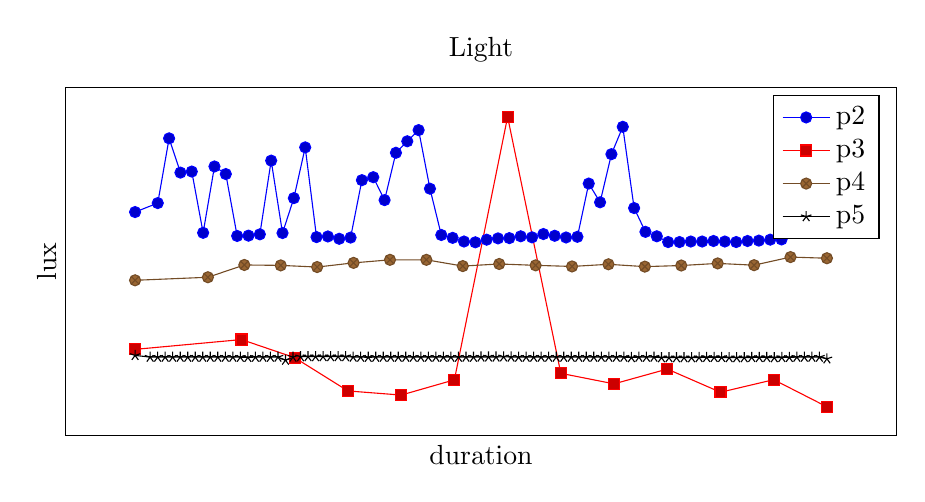
\begin{tikzpicture}
	\pgfplotsset{ticks=none}
\begin{axis}[
	height=6cm,
	width=\textwidth,
	ylabel=lux,
	xlabel=duration,
	title=Light,
	unbounded coords=discard],
	
\addplot coordinates {
(0, 372.352941176)
(2.98360655738, 389.5)
(4.47540983607, 513.25)
(5.96721311475, 447.75)
(7.45901639344, 449.75)
(8.95081967213, 332.666666667)
(10.4426229508, 459.5)
(11.9344262295, 445.0)
(13.4262295082, 326.666666667)
(14.9180327869, 327.25)
(16.4098360656, 329.75)
(17.9016393443, 470.666666667)
(19.393442623, 332.25)
(20.8852459016, 399.0)
(22.3770491803, 496.0)
(23.868852459, 324.5)
(25.3606557377, 325.666666667)
(26.8524590164, 321.25)
(28.3442622951, 323.5)
(29.8360655738, 433.333333333)
(31.3278688525, 439.0)
(32.8196721311, 395.2)
(34.3114754098, 485.666666667)
(35.8032786885, 507.666666667)
(37.2950819672, 529.0)
(38.7868852459, 417.0)
(40.2786885246, 328.5)
(41.7704918033, 323.0)
(43.262295082, 316.0)
(44.7540983607, 314.5)
(46.2459016393, 319.5)
(47.737704918, 322.0)
(49.2295081967, 322.5)
(50.7213114754, 326.0)
(52.2131147541, 324.0)
(53.7049180328, 330.333333333)
(55.1967213115, 327.0)
(56.6885245902, 323.75)
(58.1803278689, 325.0)
(59.6721311475, 426.8)
(61.1639344262, 391.0)
(62.6557377049, 483.0)
(64.1475409836, 535.333333333)
(65.6393442623, 380.0)
(67.131147541, 334.5)
(68.6229508197, 326.0)
(70.1147540984, 315.0)
(71.606557377, 315.0)
(73.0983606557, 316.0)
(74.5901639344, 316.0)
(76.0819672131, 317.0)
(77.5737704918, 316.0)
(79.0655737705, 315.0)
(80.5573770492, 317.0)
(82.0491803279, 317.75)
(83.5409836066, 319.571428571)
(85.0327868852, 320.0)
(86.5245901639, 408.684210526)
(88.0163934426, 496.0)
(89.5081967213, 474.0)
(91.0, 490.5)
};

\addplot coordinates {
(0, 109.80952381)
(14.0, 128.555555556)
(21.0, 93.8571428571)
(28.0, 30.3333333333)
(35.0, 22.4285714286)
(42.0, 51.5714285714)
(49.0, 554.333333333)
(56.0, 64.0)
(63.0, 43.875)
(70.0, 72.1666666667)
(77.0, 27.8333333333)
(84.0, 51.8571428571)
(91.0, 0.0)
};

\addplot coordinates {
(0, 241.869565217)
(9.57894736842, 247.684210526)
(14.3684210526, 271.19047619)
(19.1578947368, 270.380952381)
(23.9473684211, 267.19047619)
(28.7368421053, 275.181818182)
(33.5263157895, 281.0)
(38.3157894737, 281.0)
(43.1052631579, 269.056565454)
(47.8947368421, 273.082245)
(52.6842105263, 270.457685359)
(57.4736842105, 268.358045125)
(62.2631578947, 272.456782138)
(67.0526315789, 268.0)
(71.8421052632, 270.121246868)
(76.6315789474, 274.154865478)
(81.4210526316, 270.782398425)
(86.2105263158, 286.252546845)
(91.0, 284.054086785)
};

\addplot coordinates {
(0, 98.2916666667)
(1.97826086957, 95.0)
(2.96739130435, 95.0)
(3.95652173913, 95.0)
(4.94565217391, 95.0)
(5.9347826087, 95.0)
(6.92391304348, 95.0)
(7.91304347826, 95.0)
(8.90217391304, 95.0)
(9.89130434783, 95.0)
(10.8804347826, 95.0)
(11.8695652174, 95.0)
(12.8586956522, 95.0)
(13.847826087, 94.8825577778)
(14.8369565217, 94.5164273333)
(15.8260869565, 95.0)
(16.8152173913, 95.0)
(17.8043478261, 95.0)
(18.7934782609, 95.0)
(19.7826086957, 89.25)
(20.7717391304, 95.0078283333)
(21.7608695652, 95.7297625)
(22.75, 95.986889)
(23.7391304348, 96.0)
(24.7282608696, 96.0)
(25.7173913043, 96.0)
(26.7065217391, 96.0)
(27.6956521739, 96.0)
(28.6847826087, 95.0976655)
(29.6739130435, 95.0)
(30.6630434783, 94.678594)
(31.652173913, 95.0)
(32.6413043478, 95.0)
(33.6304347826, 95.0)
(34.6195652174, 95.0)
(35.6086956522, 95.0)
(36.597826087, 95.0)
(37.5869565217, 94.8333333333)
(38.5760869565, 95.0)
(39.5652173913, 95.0)
(40.5543478261, 95.0)
(41.5434782609, 95.0)
(42.5326086957, 95.0)
(43.5217391304, 95.0)
(44.5108695652, 95.0)
(45.5, 95.25)
(46.4891304348, 95.3285295)
(47.4782608696, 95.190542)
(48.4673913043, 95.601148)
(49.4565217391, 95.190604)
(50.4456521739, 95.0)
(51.4347826087, 95.0)
(52.4239130435, 95.0)
(53.4130434783, 95.0)
(54.402173913, 95.0)
(55.3913043478, 95.0)
(56.3804347826, 95.0)
(57.3695652174, 95.0)
(58.3586956522, 95.0)
(59.347826087, 95.0)
(60.3369565217, 95.0)
(61.3260869565, 95.0)
(62.3152173913, 95.0)
(63.3043478261, 95.0)
(64.2934782609, 95.0)
(65.2826086957, 94.2)
(66.2717391304, 95.0)
(67.2608695652, 95.0)
(68.25, 95.0)
(69.2391304348, 94.0025184211)
(70.2282608696, 94.0)
(71.2173913043, 94.0)
(72.2065217391, 94.0)
(73.1956521739, 94.0)
(74.1847826087, 94.25)
(75.1739130435, 94.6)
(76.1630434783, 94.524485)
(77.152173913, 94.5133925)
(78.1413043478, 94.0)
(79.1304347826, 94.0)
(80.1195652174, 94.0)
(81.1086956522, 94.48627)
(82.097826087, 94.3333333333)
(83.0869565217, 94.486889)
(84.0760869565, 94.0)
(85.0652173913, 94.3959052)
(86.0543478261, 94.5150075)
(87.0434782609, 95.0)
(88.0326086957, 95.0)
(89.0217391304, 95.0)
(90.0108695652, 95.0)
(91.0, 91.78003)
};

\addlegendentry{p2}
\addlegendentry{p3}
\addlegendentry{p4}
\addlegendentry{p5}
\end{axis}

\end{tikzpicture}
\caption{Environmental Light}\label{ligps}
 	\vspace{5 mm}
\end{figure}

\FloatBarrier

\subsection{Problems}
The gathering process showed some problems with the permissions of different mobile devices and different settings. Not every device has the same sensors and some devices have different default security settings that permit to access specific data within the application even when the application itself has permissions granted.

\section{Individual Experiment Results}
The results of the individual experiment are demonstrating the usage and the abilities for the Dather Application for a single participant. Rather than in the first experiment, it is taking only the data of a single person into account.
The data only shows a plausible factor but doesn't confirm the influences of the tested factors. A lot more test cases would be needed to create a more accurate average value. However, the purpose of this experiment was to demonstrate the usage of the data in more controlled comparable environments rather than in the other experiment which detected the environment and patterns. 

\subsection{coffee}
The table \ref{coffee} shows the times of 10 Sudoku solvings of the participant. The results indicates that at the beginning the participant was faster under the influence of caffeine and then in later runs it happened to be the opposite. As the measurements where done on different days, the participant probably gained more practice in solving Sodukus, which shows the decreasing time to solve a Sudoku.
\\
The average time, the participant needed without drinking coffee was \textbf{14:24 minutes} and after consuming \textbf{17:37 minutes} minutes per Sudoku. The participnat needed 3:13 minutes or 22.34\%  longer after having a strong coffee \ref{resultCoffee}.\\
These results are different than the findings in \cite{liguori1997absorption}. Their results showed that a similar amount of caffeine increases the cognitive performance. \\
However, in our case the participant of the Experiment mentioned to feel fretful after the intake of the high amount of caffeine. That could be a reason for the lower performance of the subject. Thus, it is possible that a overdose had negative impact on the participant and lower amount of caffeine would have had resulted better. 

\FloatBarrier


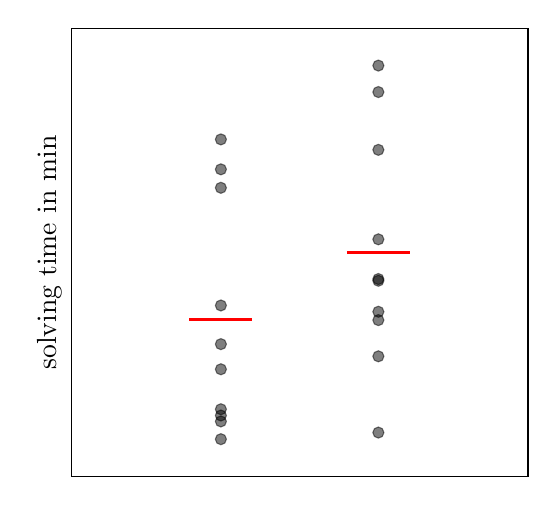
\begin{tikzpicture}
\begin{axis}[
ylabel=solving time in min,
xtick={0,1},
xticklabels={Before Coffee, After Coffee},
x=2cm,
x tick label style={rotate=45, anchor=east, align=center},
enlarge x limits={abs=1.5cm}, 
scatter/classes={%
    a={mark=*,draw=black}}]
\addplot[scatter,only marks, fill opacity=0.5, opacity=0.5, 
    scatter src=explicit symbolic]
table[meta=label] {
x 	y 						label
0	20.716667		1
0	21.6					2
0	13.233333		3
0	23.0333333	4
0	9.533333		5
0	12.03				6
0	15.0833333	7
0	9.816667		8
0	10.116667		9
0	8.683333		10
};

\addplot[mark=none, color=red, very thick] 
coordinates {
(-0.2, 14.42) 
(	0.2,14.42)
};

\addplot[scatter,only marks, fill opacity=0.5, opacity=0.5,
    scatter src=explicit symbolic]
table[meta=label] {
x 	y	 				label
1 12.65			1
1 22.533333	2
1 9.0				3
1 26.566667	4
1 14.383333	5
1 16.35			6
1 25.3				7
1 16.266667	8
1 14.783333	9
1 18.25			10
};

\addplot[mark=none, color=red, very thick] 
coordinates {
(0.8, 17.62) 
(	1.2,17.62)
};


\end{axis}
\end{tikzpicture}


%%%%%%% COFFEE Graph
\begin{figure}[ht]
	\centering
	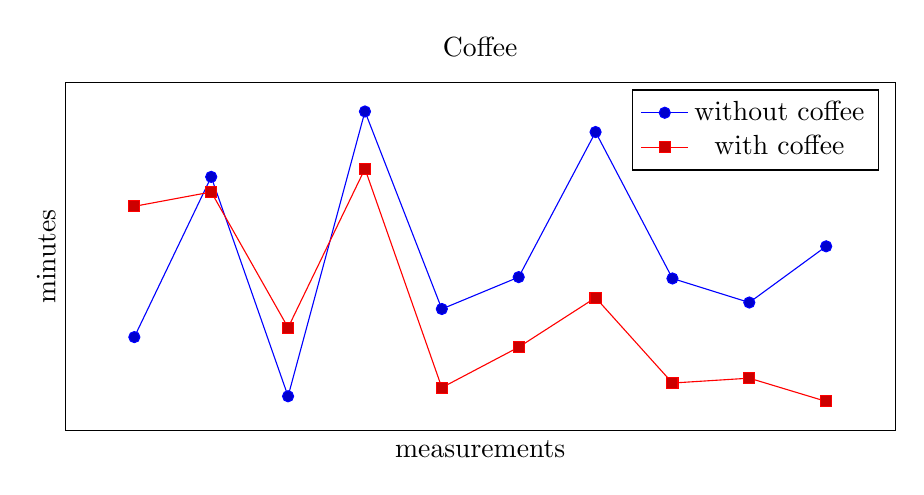
\begin{tikzpicture}
\begin{axis}[
	height=6cm,
	width=\textwidth,
	ylabel=minutes,
	xlabel=measurements,
	title=Coffee,
	unbounded coords=discard],

%Before
\addplot coordinates {
	(1, 12.65)
	(2, 22.533333)
	(3, 9.0)
	(4, 26.566667)
	(5, 14.383333)
	(6, 16.35)
	(7, 25.3)
	(8, 16.266667)
	(9, 14.783333)
	(10, 18.25)
};

\addplot coordinates {
	(1, 20.716667)
	(2, 21.6)
	(3, 13.233333)
	(4, 23.0333333)	
	(5, 9.533333)
	(6, 12.03)
	(7, 15.0833333)
	(8, 9.816667)
	(9, 10.116667)
	(10, 8.683333)
};

\addlegendentry{without coffee}
\addlegendentry{with coffee}

\end{axis}
 	\end{tikzpicture}
 	\caption{Solving times graph - Coffee}\label{resultadasda}
 	\vspace{10 mm}
\end{figure}

\FloatBarrier


% Define bar chart colors
%
\definecolor{noCoff}{HTML}{1c90e7}
\definecolor{coffee}{HTML}{a4c639}

\begin{figure}
	\centering
	\begin{tikzpicture}
        \begin{axis}[
            width  = 0.5*\textwidth,
        	height = 8cm,
        	major x tick style = transparent,
        	ybar=2*\pgflinewidth,
        	bar width=30pt,
        	ymajorgrids = true,
        	ylabel = {Average solving time},
        	symbolic x coords={Influences},
       	 	xtick = data,
        	scaled y ticks = false,
        	enlarge x limits=0.25,
        	ymin=0,
        	legend cell align=left,
        	legend style={
                at={(1,1.05)},
                anchor=south east,
                column sep=1ex
        	}
      	]
     	\addplot[style={android,fill=noCoff,mark=no coffee}]
            coordinates {(Influences, 14.42)};

        \addplot[style={ios,fill=coffee,mark=coffee}]
             coordinates {(Influences,17.62)};

        \legend{No Coffee, Coffee} 

        \end{axis}
 	\end{tikzpicture}
 	\caption{Solving times block diagram - Coffee} \label{resultCoffee}
 	\vspace{10 mm}
\end{figure}

%CONTROLL VALUE

\pgfplotsset{every error bar/.style={line width=1 cm}}

\pgfplotstableread{
x         				y    			y-max  				y-min
BeforeCoffee  	14.42		23.0333333  	8.683333  
AfterCoffee  	17.62  		26.566667  	9.0
}{\mytable}

\begin{tikzpicture}[scale=1.3] 
\begin{axis} [
	width  = 0.5*\textwidth,
	height = 8cm,
	x=2cm,
	enlarge x limits={abs=1.5cm}, % The distance between the center of the first bar and the left edge
	symbolic x coords={BeforeCoffee, AfterCoffee},
	x tick label style={rotate=45, anchor=east, align=center},
	xtick=data,
    ymajorgrids = true,
    ylabel = {Average solving time},
    scaled y ticks = false,
    ymin=0,
    legend cell align=left,
    legend style={
    	at={(1,1.05)},
      	anchor=south east,
       column sep=1ex
    }
]
\addplot+[blue, very thick, forget plot,only marks] 
  plot[very thick, error bars/.cd, y dir=plus, y explicit]
  table[x=x,y=y,y error expr=\thisrow{y-max}] {\mytable};
\addplot+[red, very thick, only marks,xticklabels=\empty] 
  plot[very thick, error bars/.cd, y dir=minus, y explicit]
  table[x=x,y=y,y error expr=\thisrow{y-min}] {\mytable};
\end{axis} 
\end{tikzpicture}





\FloatBarrier

\subsection{music}

\ref{resultMusicGraph} and \ref{resultMusic} show the times of the Sudokus that have been solved by the participant and the duration it took. It shows that the average time of solving was the shortest when the participant was listening to music. 
The participant solved the ten Sudokus in 89.35\% of the average time compared to the results archived without music. That is 1 minute and 34 seconds less time in average. 
On the other hand, the average solving time while listening to heavy metal music was 4.08 \% or 36 seconds slower than without listening to music. 
The results show evidence that for the participant the cognitive performance in solving Sudoku riddles was increasing when listening to classical music and decreasing at heavy metal music. 

\FloatBarrier

%%%%%%% Music
\begin{figure}[ht]
	\centering
	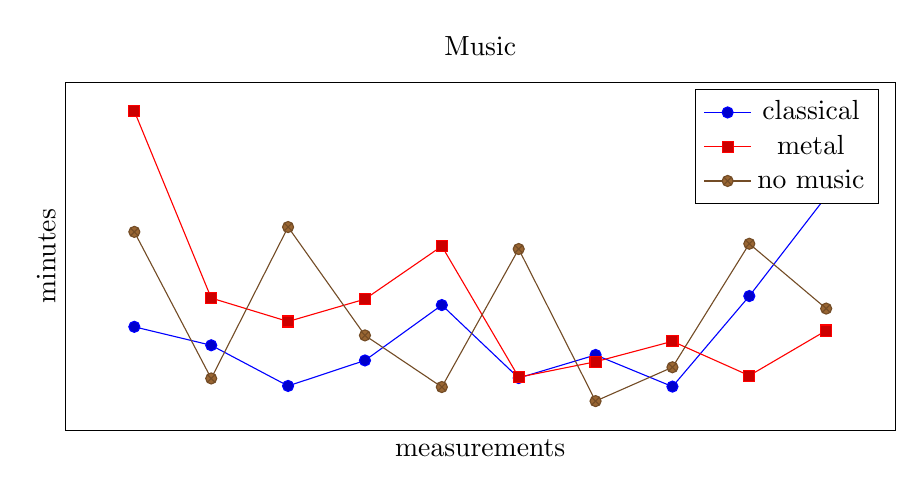
\begin{tikzpicture}
\begin{axis}[
	height=6cm,
	width=\textwidth,
	ylabel=minutes,
	xlabel=measurements,
	title=Music,
	unbounded coords=discard],

% classical
\addplot coordinates {
	(1, 13.666667)
	(2, 12.266667)
	(3, 9.183333)
	(4, 11.116667)
	(5, 15.316667)
	(6, 9.783333)
	(7, 11.533333)
	(8, 9.133333)
	(9, 16.0)
	(10, 23.55)
};

% metal
\addplot coordinates {
	(1, 30.02)
	(2, 15.85)
	(3, 14.07)
	(4, 15.766667)
	(5, 19.783333)
	(6, 9.85)
	(7, 11.0166667)
	(8, 12.566667)
	(9, 9.966667)
	(10, 13.383333)
};

% none
\addplot coordinates {
	(1, 20.866667)
	(2, 9.75)
	(3, 21.233333)
	(4, 13.0166667)
	(5, 9.1)
	(6, 19.566667)
	(7, 8.0333333)
	(8, 10.6)
	(9, 19.966667)
	(10, 15.05)
};

\addlegendentry{classical}
\addlegendentry{metal}
\addlegendentry{no music}

\end{axis}
 	\end{tikzpicture}
 	\caption{Solving times graph - Music}\label{resultMusicGraph}
 	\vspace{10 mm}
\end{figure}


% Define bar chart colors
%
\definecolor{nada}{HTML}{e78d1c}
\definecolor{metal}{HTML}{a4c639}
\definecolor{classical}{HTML}{1c90e7}

\begin{figure}
	\centering
	\begin{tikzpicture}
        \begin{axis}[
            width  = 0.5*\textwidth,
        	height = 8cm,
        	major x tick style = transparent,
        	ybar=2*\pgflinewidth,
        	bar width=30pt,
        	ymajorgrids = true,
        	ylabel = {Average solving time},
        	symbolic x coords={Influences},
       	 	xtick = data,
        	scaled y ticks = false,
        	enlarge x limits=0.25,
        	ymin=0,
        	legend cell align=left,
        	legend style={
                at={(1,1.05)},
                anchor=south east,
                column sep=1ex
        	}
      	]
     	\addplot[style={android,fill=classical,mark=classical}]
            coordinates {(Influences, 13.15)};

        \addplot[style={ios,fill=,metal,mark=metal}]
             coordinates {(Influences,15.316667)};

        \addplot[style={others,fill=nada,mark=no music}]
             coordinates {(Influences, 15.005)};

        \legend{Classical, Metal, No Music} 

        \end{axis}
 	\end{tikzpicture}
 	\caption{Solving times block diagram - Music}\label{resultMusic}
 	\vspace{10 mm}
\end{figure}

\FloatBarrier

\subsection{running}
The graph \ref{resultRun} results show a trend for a better performance after strong physical activity. The average solving time after the run (\textbf{10:52 min}) is 3:20 min faster than the \textbf{14:12} minutes before running. That is a decrease of \textbf{22.5\%} from before to after and can be seen in \ref{resultRunning}. 
Compared to the two other individual experiments, the results of this scenario are differing more at each measurement. 4 times, the solving after the running took actually longer than the solvings in the pre-run state. 

%%%%%%% Running
\begin{figure}[ht]
	\centering
	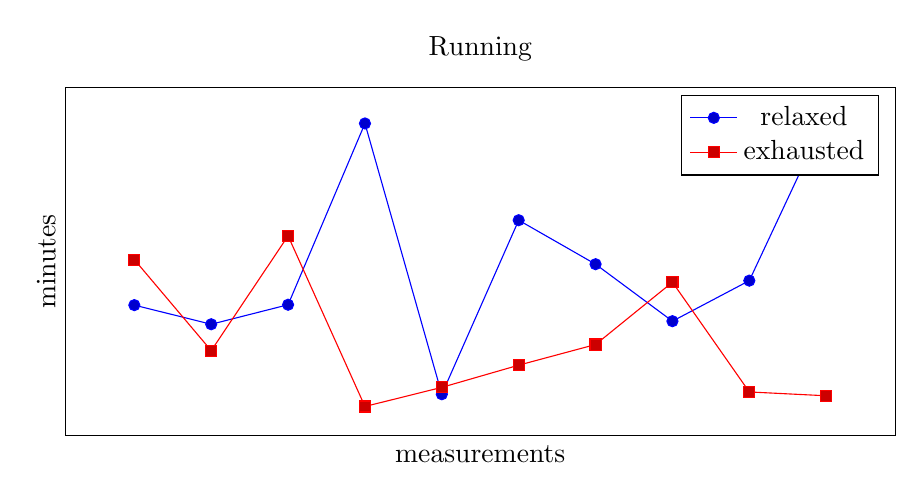
\begin{tikzpicture}
\begin{axis}[
	height=6cm,
	width=\textwidth,
	ylabel=minutes,
	xlabel=measurements,
	title=Running,
	unbounded coords=discard],

\addplot coordinates {
	(1, 12.466667)
	(2, 11.633333)
	(3, 12.483333)
	(4, 20.383333)
	(5, 8.583333)
	(6, 16.166667)
	(7, 14.25)
	(8, 11.766667)
	(9, 13.533333)
	(10, 20.683333)
};

\addplot coordinates {
	(1, 14.45)
	(2, 10.483333)
	(3, 15.483333)
	(4, 8.05)
	(5, 8.883333)
	(6, 9.85)
	(7, 10.75)
	(8, 13.466667)
	(9, 8.683333)
	(10, 8.516667)
};

\addlegendentry{relaxed}
\addlegendentry{exhausted}

\end{axis}
 	\end{tikzpicture}
 	\caption{Solving times graph - Running}\label{resultRun}
 	\vspace{10 mm}
\end{figure}

\FloatBarrier

% Define bar chart colors
%
\definecolor{nada}{HTML}{e78d1c}
\definecolor{metal}{HTML}{a4c639}
\definecolor{classical}{HTML}{1c90e7}

\begin{figure}
	\centering
	\begin{tikzpicture}
        \begin{axis}[
            width  = 0.5*\textwidth,
        	height = 8cm,
        	major x tick style = transparent,
        	ybar=2*\pgflinewidth,
        	bar width=30pt,
        	ymajorgrids = true,
        	ylabel = {Average solving time},
        	symbolic x coords={Influences},
       	 	xtick = data,
        	scaled y ticks = false,
        	enlarge x limits=0.25,
        	ymin=0,
        	legend cell align=left,
        	legend style={
                at={(1,1.05)},
                anchor=south east,
                column sep=1ex
        	}
      	]
     	\addplot[style={android,fill=classical,mark=classical}]
            coordinates {(Influences, 14.02)};

        \addplot[style={ios,fill=,metal,mark=metal}]
             coordinates {(Influences,10.866667)};

        \legend{Relaxed, Exhausted} 

        \end{axis}
 	\end{tikzpicture}
 	\caption{Solving time block diagram - Running}\label{resultRunning}
 	\vspace{10 mm}
\end{figure}

\FloatBarrier
